% !TEX encoding = UTF-8 Unicode

\documentclass[a4paper]{article}

\usepackage{color}
\usepackage{listings}
\usepackage{url}
\usepackage[T2A]{fontenc} % enable Cyrillic fonts
\usepackage[utf8]{inputenc} % make weird characters work
\usepackage{graphicx}

\usepackage[english,serbian]{babel}
%\usepackage[english,serbianc]{babel} %ukljuciti babel sa ovim opcijama, umesto gornjim, ukoliko se koristi cirilica

\usepackage[unicode]{hyperref}
\hypersetup{colorlinks,citecolor=green,filecolor=green,linkcolor=blue,urlcolor=blue}

%\newtheorem{primer}{Пример}[section] %ćirilični primer
\newtheorem{primer}{Primer}[section]

\begin{document}

\title{Uvod u programiranje\\ \small{Skipta za kurs\\Uvod u programiranje kroz JavaScript\\}}

\author{Una Stanković\\ unastankovic1310@gmail.com}
\date{10.~septembar 2018.}
\maketitle
\newpage

U ovom tekstu predstavljene su teorijske osnove potrebne za savladavanje kursa $"$ Uvod u programiranje kroz JavaScript$"$. Najpre su navedene, ukratko, teorijske osnove računarstva i uvod kroz HTML i CSS, a kasnije se ulazi u rad sa JavaScript-om.  Ova skripta je obavezan materijal pri kursu i sa prezentacijama i kodovima formira celinu. Ova skripta sama po sebi nije dovoljna, samostalan rad i istraživanje je neizostavni deo procesa učenja. U slučaju da primetite greške pri čitanju rada ili imate bilo kakve nedoumice, predloge i sugestije javite se mejlom na adresu navedenu na prvoj strani.

\newpage

\tableofcontents

\newpage

\section{Uvod u računarstvo}
\label{sec:uvod}
Računarstvo i informatika predstavljaju jednu od najvažnijih oblasti današnjice koje su u konstantnom razvoju. Danas, ne možemo zamisliti život bez računara, pametnih telefona ili mnogobrojnih uređaja koji se pokreću uz pomoć računara. Razvitak računarstva i tehnologije u poslednjih 70 godina je eksponencijalan, tako da, danas, imamo razvoj prenosnih računara, tableta, pametnih telefona i uređaja, kola, kućnih aparata i ostalih koji se pokreću korišćenjem računarskih sistema. Kako definisati računarski sistem? Postoji više različitih računarskih sistema, od kojih svaki ima svoju posebnu definiciju, ali naš fokus je na digitalnim računarskim sistemima. Oni podrazumevaju mašinu koja može da se programira kako bi izvršavala različite zadatke svođenjem na elementarne operacije nad brojevima. Brojevi se u računaru zapisuju uz pomoć nula i jedinica, odnosno, binarnim zapisom, kao nizovi bitova. \\\\
Kada se razmišlja o tome šta sve računarstvo obuhvata, lako se uviđa da računarstvo nije samo računar, već da ono predstavlja mnogo širu oblast koja se bavi izučavanjem teorije i prakse procesa računanja i primene računara u različitim naučnim oblastima, tehnici i svakodnevnom životu. Računar sam po sebi nije cilj, već sredstvo za postizanje različitih ciljeva u zavisnosti od njihove primene. Za današnje računare često ćemo čuti da su $"$programabilni$"$, ali šta to zapravo govori? Programabilnost računara se ogleda u činjenici da je moguće računaru dati neki skup instrukcija koje će on izvršavati sa ciljem ispunjavanja određenih zadataka, koje mu čovek, odnosno, programer zadaje. Računari kakve danas poznajemo nastali su polovinom XX veka, ali želja za automatizacijom određenih postupaka seže daleko dalje u prošlost. Naime, posmatrajući istorijski, ljudi su vekovima stvarali razne naprave koje su mogle da rešavaju neke numeričke zadatke. 

\subsection{Istorijat računarstva}
Da bismo u potpunosti razumeli računarstvo moramo imati uvid u njegove početke i razvoj.
 
\subsection{Fon Nojmanova arhitektura}
Na osnovu istorijata može se uočiti da svi navedeni računari imaju nedostatak jedne važne karakteristike računara danas, a to je programabilnost. Mašine korišćene nekada nisu bile programabilne već su funkcionisale po unapred definisanom programu određenom samom konstrukcijom mašine. Iako ovakav pristup nije sasvim izumro (danas se može videti na primeru digitrona), uglavnom nije poželjan. Prava promena u pristupu, koja je dovela do stvaranja programabilnih računara, nastala je ranih 1940-ih godina sa pojavom računara koji bi programe koje izvršavaju čuvali u memoriji zajedno sa podacima. Takve računare nazivamo računarima sa skladištenim podacima (engl. stored program computers). Jedna od najvažnijih karakteristika ovih računara je da kod njih postoji jasna podela na hardver i softver. Za rodonačelnika ovakve arhitekture smatra se Džon fon Nojman. On je 1945. godine opisao arhitekturu čija je glavna karakteristika da se programi mogu učitavati isto kao i podaci koji se obrađuju. Primeri prvih ovakvih računara su EDVAC, Mark 1 i EDSAC.\\\\
Osnovni elementi fon Nojmanove arhitekture su:
\begin{enumerate}
\item procesor - koji čine aritmetičko-logička jedinica, kontrolna jedinica i registri, i 
\item glavna memorija 
\end{enumerate}
koji su međusobno povezani, dok se ostale komponente računara smatraju pomoćnim. Prikaz Fon Nojmanove arhitekture je na slici \ref{fig:fonN}.
\begin{figure}[h!]
\begin{center}
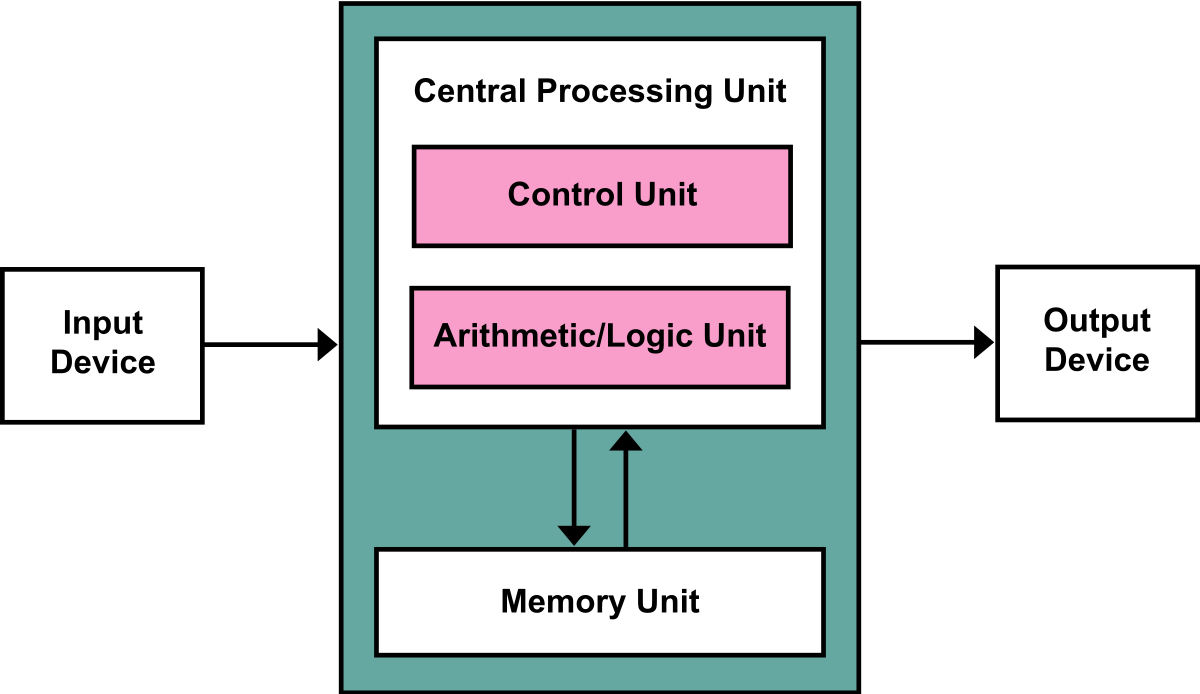
\includegraphics[scale=0.25]{pictures/fonN.png}
\end{center}
\caption{Šematski prikaz Fon Nojmanove arhitekture}
\label{fig:fonN}
\end{figure}
Pod pomoćne komponente ubrajamo ulazno-izlazne jediice, spoljašnje memorije itd., koje da bi funkcionisale moraju biti povezane na centralni deo računara (procesor i glavnu memoriju).
Osnovna uloga procesora je obrada podataka, dok je osnovna uloga memorije skladištenje podataka koji se obrađuju, kao i programa. Postoji jedinstven način na koji zapisujemo i podatke i programe, a to je uz pomoć nula i jedinica, odnosno, binarnim zapisom. Tokom rada računara podaci i programi se prenose između procesora i glavne memorije.
\subparagraph{Procesor} Prva centralna komponenta Fon Nojmanove arhitekture. Procesor, koji je odgovoran za rad računara, sastoji se od \textit{kontrolne jedinice} - koja upravlja radom procesora i \textit{aritmetičko-logičke jedinice} - koja je zadužena za izvođenje aritmetičkih operacija (sabiranje, oduzimanje, množenje, poređenje, itd. ) i logičkih operacija (konjunkcija, negacija, itd. ) nad brojevima. Osim dva navedena dela procesor sadrži i određeni broj registara, obično fiksirane širine (8, 16, 32 ili 64 bita), koji privremeno mogu da čuvaju podatke. Danas procesori neretko poseduju više jezgara (engl. core) koja istovremeno izvršavaju instrukcije čime se obezbeđuje paralelno izvršavanje.
\subparagraph{Memorija} Druga centralna komponenta Fon Nojmanove arhitekture
je glavna memorija. Memorija predstavlja linearno uređeni niz registara, pri čemu svaki ima svoju adresu. Kao posledica osobine ove memorije da se sadržaju može pristupati u slučajnom redosledu, čest naziv je i memorija sa slobodnim pristupom (engl. RAM - random access memory). Razlikujemo nekoliko parametara koji odlikuju memoriju, to su:
\begin{itemize}
\item kapacitet - GB,
\item vreme pristupa - vreme potrebno da se memorija pripremi za čitanje ili upis i 
\item protok - izražava količinu podataka koji se prenose po jedinici merenja (danas obično mereno u GBps).
\end{itemize}
Na slici \ref{fig:memh} može se videti memorijska hijerarhija.
\begin{figure}[h!]
\begin{center}
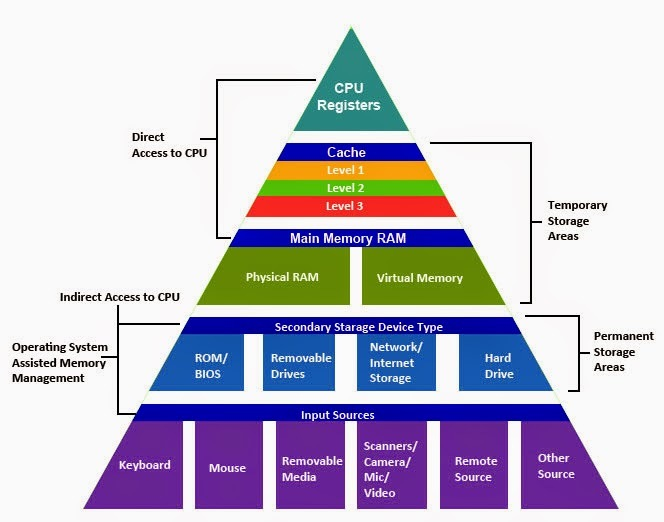
\includegraphics[scale=0.25]{pictures/mem_hijer.jpg}
\end{center}
\caption{Šematski prikaz memorijske hijerarhije}
\label{fig:memh}
\end{figure}

\subsection{Hardver}
Bez obzira na činjenicu da osnovu savremenih računarskih sistema i dalje čini Fon Nojmanova arhitektura, za rad računara u današnjem smislu reči potreban je i čitav niz hardverskih komponenti koje nam dodatno olakšavaju. Opis komponenti koje čine jedan računar danas ne sastoji se od kućišta, monitora, tastature i miša, već nam je potreban apstraktniji, sveobuhvatniji opis. Upravo, kako bi se jasnije i preciznije opisao računar kaže se da ga čine:
\begin{itemize}
\item procesor tj. centralna procesorska jedinica (engl. Central Processing Unit,
CPU), koja obrađuje podatke,
\item glavna memorija (engl. main memory), u kojoj se istovremeno čuvaju i
podaci koji se obrađuju i trenutno pokrenuti programi, i 
\item različiti periferijski uređaji ili ulazno-izlazne jedinice (engl. peripherals,
input-output devices, IO devices), u koje se ubrajaju miševi, tastature, ekrani,
štampači, diskovi, a koji služe za interakciju između korisnika i sistema i trajno skladištenje podataka i programa.
\end{itemize} 
Da bi se izvršilo povezivanje svih navedenih komponenti koristimo magistralu.
Za funkcionisanje modernih računara neophodni su i hardver i softver. 
Hardver (tehnički sistem računara) čine opipljive, fizičke komponente računara: procesor, memorija, matična ploča, itd. 

\subsection{Softver}
Softver računara čine programi i prateći podaci koji određuju izračunavanja koja vrši računar.
Prvi računari su se odlikovali jezicima specifičnim za konkretni računar - mašinski zavisnim jezicima. Već od 1950-ih, sa pojavom prvih jezika višeg nivoa, programiranje postaje dosta lakše. Danas, programi se najčešće pišu u višim programskim jezicima, a potom se prevode na mašinski jezik, onaj koji je razumljiv računaru. Programom opisujemo računaru koje operacije treba da izvrši sa ciljem ispunjavanja nekog zadatka. U nastavku biće navedeno nekoliko primera koji ilustruju izvršavanje programa napisanih na višim programskim jezicima. 
\begin{primer}
Želimo da izračunamo vrednost izraza $2*x + 3$ za neko $x$. Podatke u računarstvu, kao i u matematici, možemo predstaviti pomoću promenljivih. Međutim, za razliku od matematike, promenljive u računarstvu mogu menjati svoju vrednost. Svakoj promenljivoj je u memoriji računara pridruženo jedno fiksirano mesto i ona može tokom izvršavanja programa da menja vrednost. Recimo da je $x$ ulazni parametar našeg programa, a $y$ izlazna vrednost, tada izračunavanje opisujemo sa
\begin{verbatim}
y := 2*x + 3
\end{verbatim}
gde $*$ označava množenje, $+$ sabiranje, a $:=$ naredbu dodele, odnosno promenljivoj sa leve strane izraza dodeljujemo vrednost izraza sa desne strane.
\end{primer}
\begin{primer}
Kao naredni primer uzmimo poređenje dva broja, odnosno, kao izlaz treba da dobijemo veći od dva broja.
Ovakav izraz možemo zapisati kao:
\begin{verbatim}
ako je x >= y onda
m := x
inače
m := y
\end{verbatim}
\end{primer}
\begin{primer}
Kao još jedan primer uzmimo stepenovanje:
\begin{verbatim}
s := 1, i := 0
dok je i < n radi sledeće:
s := s·x, i := i + 1
\end{verbatim}
\end{primer}
Savremeni softver klasifikujemo u 2 kategorije:
\begin{itemize}
\item Sistemski i
\item Aplikativni.
\end{itemize}
\textbf{\em Aplikativni softver} je onaj koji krajnji korisnici računara direktno koriste u svojim svakodnevnim aktivnostima. Tu spadaju, na primer, pregledači Veba, e-mail klijenti, kancelarijski softver (programi za kucanje teksta, izradu prezentacija,...), video igre, softver za prikaz slika, itd.\\
\textbf{\em Sistemski softver} ima ulogu da kontroliše hardver i pruža usluge aplikativnom softveru. Najznačajniji skup sistemskog softvera je operativni sistem (OS), ali u sistemski softver ubrajamo i različite uslužne programe: editore teksta, alate za programiranje (prevodioci, dibageri, profajleri, integrisana okruženja) i slično. Uloga operativnog sistema je da programeru pruži skup funkcija koje programer može da koristi kako bi ispunio određeni cilj, sakrivajući konkretne hardverske detalje - ovaj skup funkcija naziva se programski interfejs za pisanje aplikacija (engl. API - Application Programming Interface).

\subsection{Oblasti savremenog računarstva}
Savremeno računarstvo sastoji se iz više podoblasti između kojih nema jasnih granica. Prema klasifikaciji američke asocijacije ACM - Association for Computing Machinery, razlikujemo naredne podoblasti~\cite{Janicic}:
\begin{itemize}
\item Algoritmika (procesi izračunavanja i njihova složenost)
\item Strukture podataka (reprezentovanje i obrada podataka)
\item Programski jezici (dizajn i analiza svojstava formalnih jezika za opisivanje
algoritama)
\item Programiranje (proces zapisivanja algoritama u nekom programskom jeziku)
\item Softversko inženjerstvo (proces dizajniranja, razvoja i testiranja programa)
\item Prevođenje programskih jezika (efikasno prevođenje viših programskih jezika,
obično na mašinski jezik)
\item Operativni sistemi (sistemi za upravljanje računarom i programima)
\item Mrežno računarstvo (algoritmi i protokoli za komunikaciju između računara)
\item Primene (dizajn i razvoj softvera za svakodnevnu upotrebu)
\item Istraživanje podataka (pronalaženje relevantnih informacija u velikim skupovima
podataka)
\item Veštačka inteligencija (rešavanje problema u kojima se javlja kombinatorna
eksplozija)
\item Robotika (algoritmi za kontrolu ponašanja robota)
\item Računarska grafika (analiza i sinteza slika i animacija)
\item Kriptografija (algoritmi za zaštitu privatnosti podataka)
\item Teorijsko računarstvo (teorijske osnove izračunavanja, računarska matematika,
verifikacija softvera, itd).
\end{itemize}

\subsection{Programiranje, algoritmi i složenost}
Programiranje predstavlja proces zapisivanja algoritama u nekom programskom jeziku. Algoritam predstavlja precizan opis postupka za rešavanje nekog problema u konačnom broju koraka. Algoritmi se odlikuju svojom složenošću. Ta složenost može biti vremenska ili memorijska. Cilj analize algoritama je predvidjanje njegovog ponašanja i brzine izvršavanja bez realizacije na nekom konkretnom računaru. Ta procena treba da se odnosi na svaki računar. Nemoguće bi bilo na svakom računaru ispitati izvršavanje nekog algoritma. Zbog toga se smatra da je analiza algoritama približna.~\cite{Zivkovic}

\newpage

\section{Uvod u web}
\label{sec:uvodweb}



\newpage
\section{HTML i CSS}
\label{sec:uvod}

\begin{primer}
 Da bi se ispitivala ispravost softvera, najpre je potrebno precizno definisati njegovo ponašanje \cite{laski2009software}. 
\end{primer}


%\begin{primer} Ovako se ubacuje slika. Obratiti pažnju da je dodato i 
%\begin{verbatim}
%\usepackage{graphicx}
%\end{verbatim}

%\begin{figure}[h!]
%\begin{center}
%\includegraphics[scale=0.75]{panda.jpg}
%\end{center}
%\caption{Pande}
%\label{fig:pande}
%\end{figure}

%Na svaku sliku neophodno je referisati se negde u tekstu. Na primer, na slici \ref{fig:pande} prikazane su pande. 
%\end{primer}

%\begin{primer} I tabele treba da budu u svom okruženju, i na njih je neophodno referisati se u tekstu. Na primer, u tabeli \ref{tab:tabela1} su prikazana različita poravnanja u tabelama.

%
%\begin{table}[h!]
%\begin{center}
%\caption{Razlčita poravnanja u okviru iste tabele ne treba koristiti jer su nepregledna.}
%\begin{tabular}{|c|l|r|} \hline
%centralno poravnanje& levo poravnanje& desno poravnanje\\ \hline
%a &b&c\\ \hline
%d &e&f\\ \hline
%\end{tabular}
%\label{tab:tabela1}
%\end{center}
%\end{table}

%\end{primer}


\section{Zaključak}
\label{sec:zakljucak}

\addcontentsline{toc}{section}{Literatura}
\appendix
\bibliography{seminarski} 
\bibliographystyle{plain}

\appendix
\section{Dodatak}


\end{document}
